\documentclass[12pt,a4paper]{scrartcl}
\usepackage{forest}
\usepackage{booktabs}
\usepackage{hyperref}
\usepackage{placeins}
\usepackage{titling}
\usepackage{graphicx}
\graphicspath{{figures/}{../figures/}}
\renewcommand{\subtitle}[1]{%
  \posttitle{%
    \par\end{center}
    \begin{center}\large#1\end{center}
    \vskip0.5em}%
}
\title{Laminar fMRI pipeline}
\author{Tommy Clausner}
\subtitle{\textsc{Documentation}}
\date{\small{last updated on \today}}

\begin{document}
\begin{titlepage}
\clearpage\maketitle
\thispagestyle{empty}
\end{titlepage}
\tableofcontents
\newpage
\listoffigures
\newpage
\listoftables
\newpage
\section{Pre- requisites}
\begin{itemize}
\item MRIcron (\href{https://www.nitrc.org/projects/mricron}{https://www.nitrc.org/projects/mricron})
\item FSL (\href{https://fsl.fmrib.ox.ac.uk/fsl/fslwiki}{https://fsl.fmrib.ox.ac.uk/fsl/fslwiki})
\item FreeSurfer (\href{https://surfer.nmr.mgh.harvard.edu/}{https://surfer.nmr.mgh.harvard.edu/})
\item MrVista (\href{https://web.stanford.edu/group/vista/cgi-bin/wiki/index.php/MrVista}{https://web.stanford.edu/group/vista/cgi-bin/wiki/index.php/MrVista})
\item SPM (\href{http://www.fil.ion.ucl.ac.uk/spm/}{http://www.fil.ion.ucl.ac.uk/spm/})
\item analysePRF (\href{http://kendrickkay.net/analyzePRF/}{http://kendrickkay.net/analyzePRF/})
\item knkutils (\href {https://github.com/kendrickkay/knkutils/}{https://github.com/kendrickkay/knkutils/})
\item Open fMRI Analysis (\href{https://github.com/TimVanMourik/OpenFmriAnalysis}{https://github.com/TimVanMourik/OpenFmriAnalysis})
\item MATLAB R2015a or later (\href{https://nl.mathworks.com/products/matlab.html}{https://nl.mathworks.com/products/matlab.html})
\item MATLAB Robotic Systems Toolbox (\href{https://nl.mathworks.com/products/robotics.html}{https://nl.mathworks.com/products/robotics.html} - can hopefully be omitted in future releases)
\end{itemize}

Use e.g. MRIcron's dicom2nii to convert raw MRI data to NifTi files.\\

It might be necessary to modify initMrVista.m such that the first two lines point towards the mrVista and SPM master directory.

\section{Folder structure}
The general folder structure is set up by a call to setupfolders.sh (see also Figure \ref{tree:folderstruct})
\begin{itemize}
\item Functional data must be located in niftis/\textbf{functionals}/
\item Anatomical data must be located in niftis/\textbf{t1}/
\item Inverted functional data must be located in niftis/\textbf{inverted}/
\item Proton density data must be located in niftis/\textbf{pd}/
\item Inverted proton density data must be located in niftis/\textbf{pdinverted}/
\end{itemize}

\section{How things work}
Parts of the analysis run in Bash shell scripts. Those can be called from their root directory using "sh scriptname.sh" (excl. quotation marks). Each step within the analysis has a different subfolder containing the respective results of this step. Leading numbers indicate in which logical order the corresponding shell scripts should be executed. Note that all files created by each respective step is stored in the coresponding folder. However files that need to be preset (e.g. config files) must be located in A\_helperfiles.\\

\noindent All functions with the prefix \textit{do\_} will affect the data.

\section{Suggested order of operations}
\subsection{Pre-processing}
\begin{itemize}
\item makenewsubject.sh (double click)
\item copy NifTi files to the correct location (see above)
\item open terminal (the following are terminal commands)
\item cd PATH/SUBJECTFOLDER/B\_scripts
\item sh runonqsub.sh 32gb do\_preparefunctionals.sh
\item sh runonqsub.sh 16gb do\_fsrecon.sh
\item sh runonqsub.sh 16gb do\_makemasksandlabels.sh
\item sh runonqsub.sh 32gb do\_realignment.sh
\item sh runonqsub.sh 16gb do\_preparecoregistration.sh
\item sh do\_correctavgdiff.sh 0.975
\item sh do\_coregistration.sh
\item sh runonqsub.sh 32gb do\_distcorr.sh
\item sh do\_prepareapplytopup.sh
\item sh runonqsub.sh 64gb do\_applydistcorr.sh
\end{itemize}
\begin{figure}[h]
\begin{center}
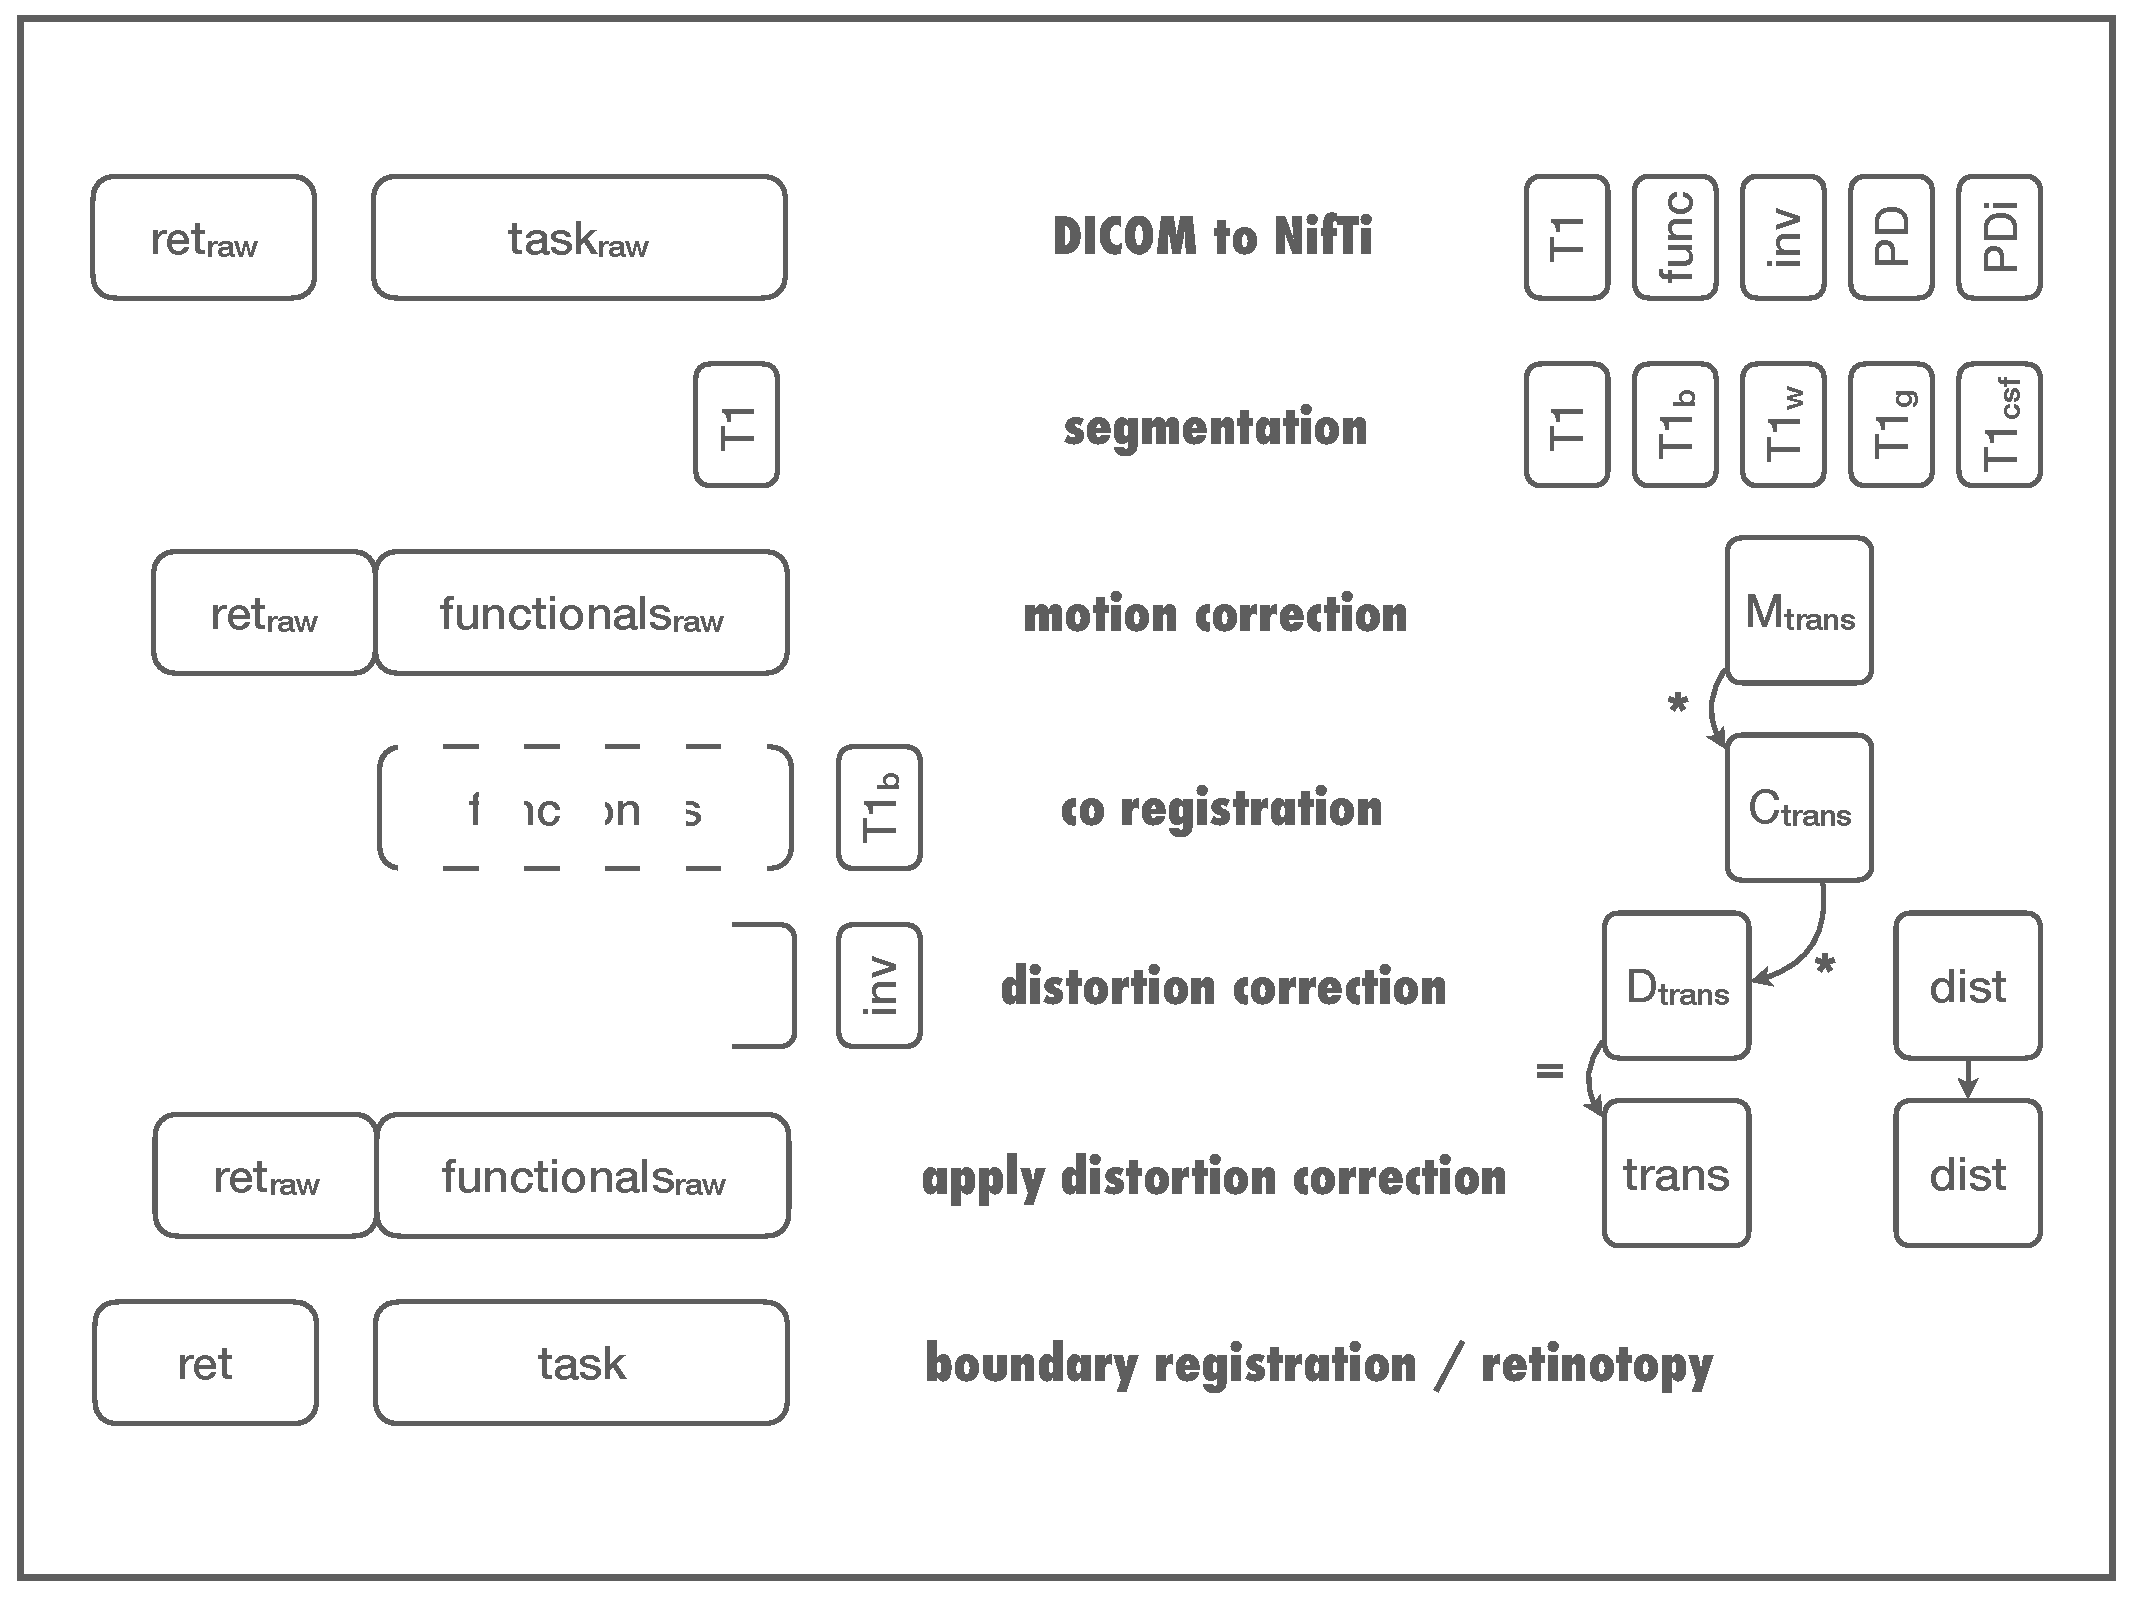
\includegraphics[width=0.8\textwidth]{overviewpreprocmain}
\caption[Overview Pre-processing fMRI]{Overview Pre-processing fMRI}
\end{center}
\end{figure}
\begin{figure}[h]
\begin{center}
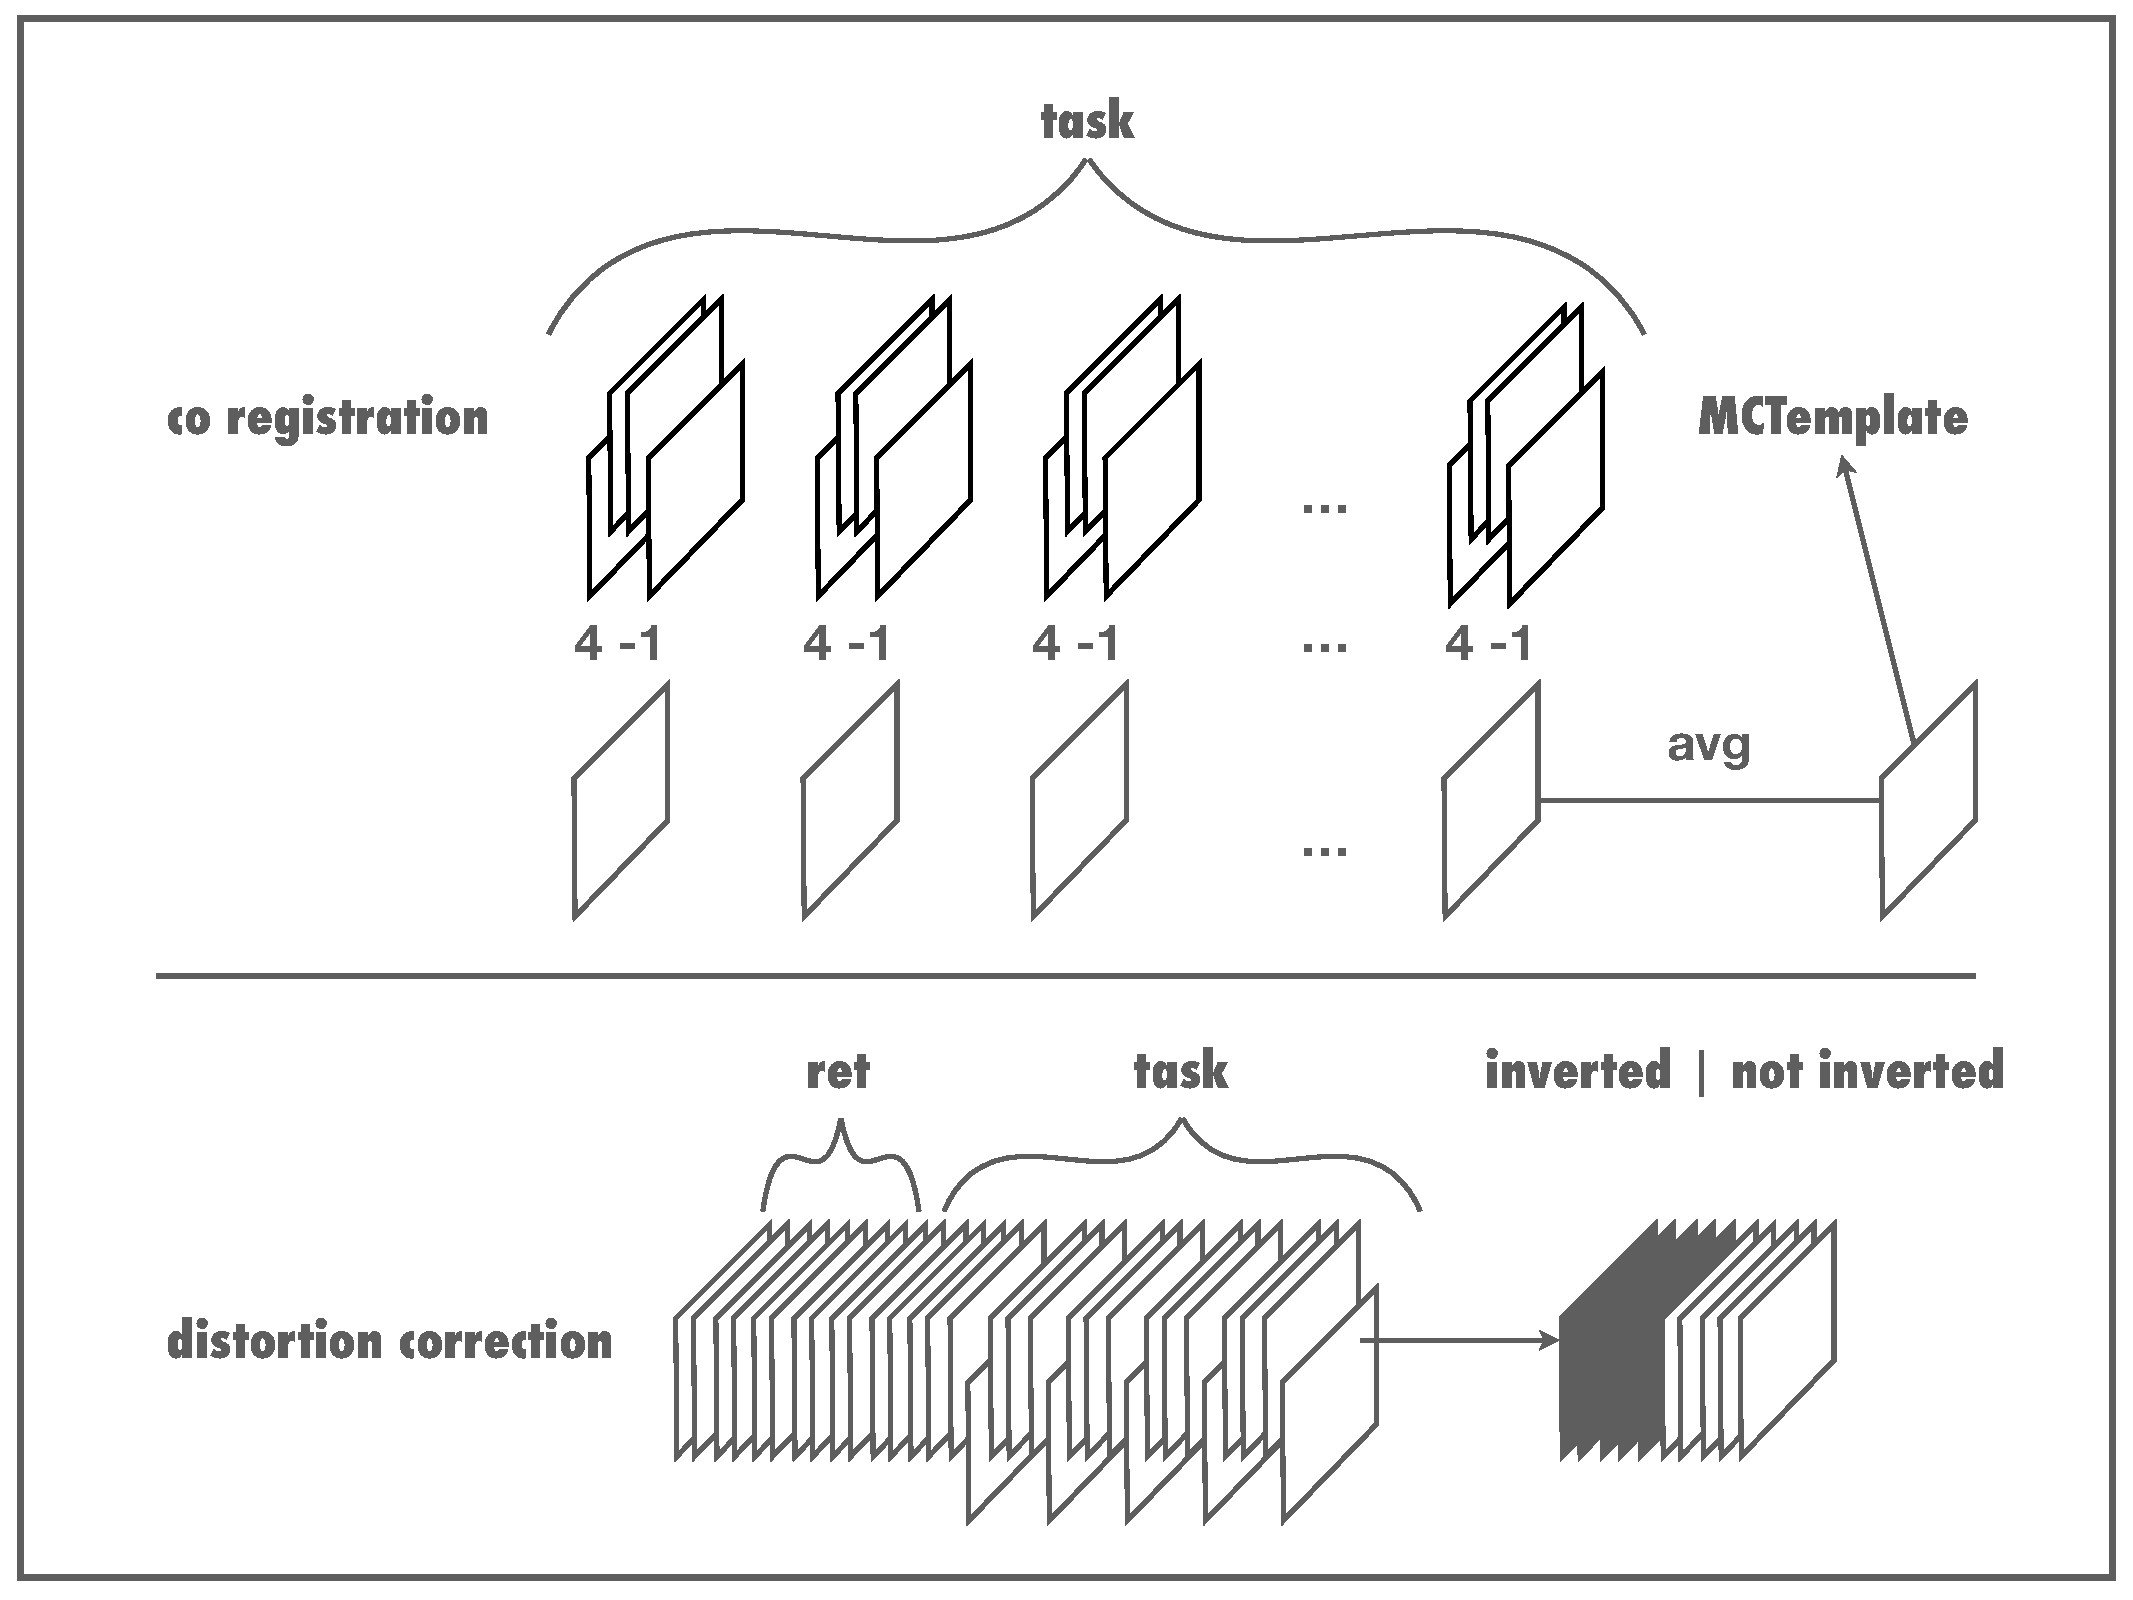
\includegraphics[width=0.8\textwidth]{coregdist}
\caption[Coregistration and distortion correction visual depiction]{Coregistration and distortion correction visual depiction}
\end{center}
\end{figure}
\begin{figure}[h]
\begin{center}
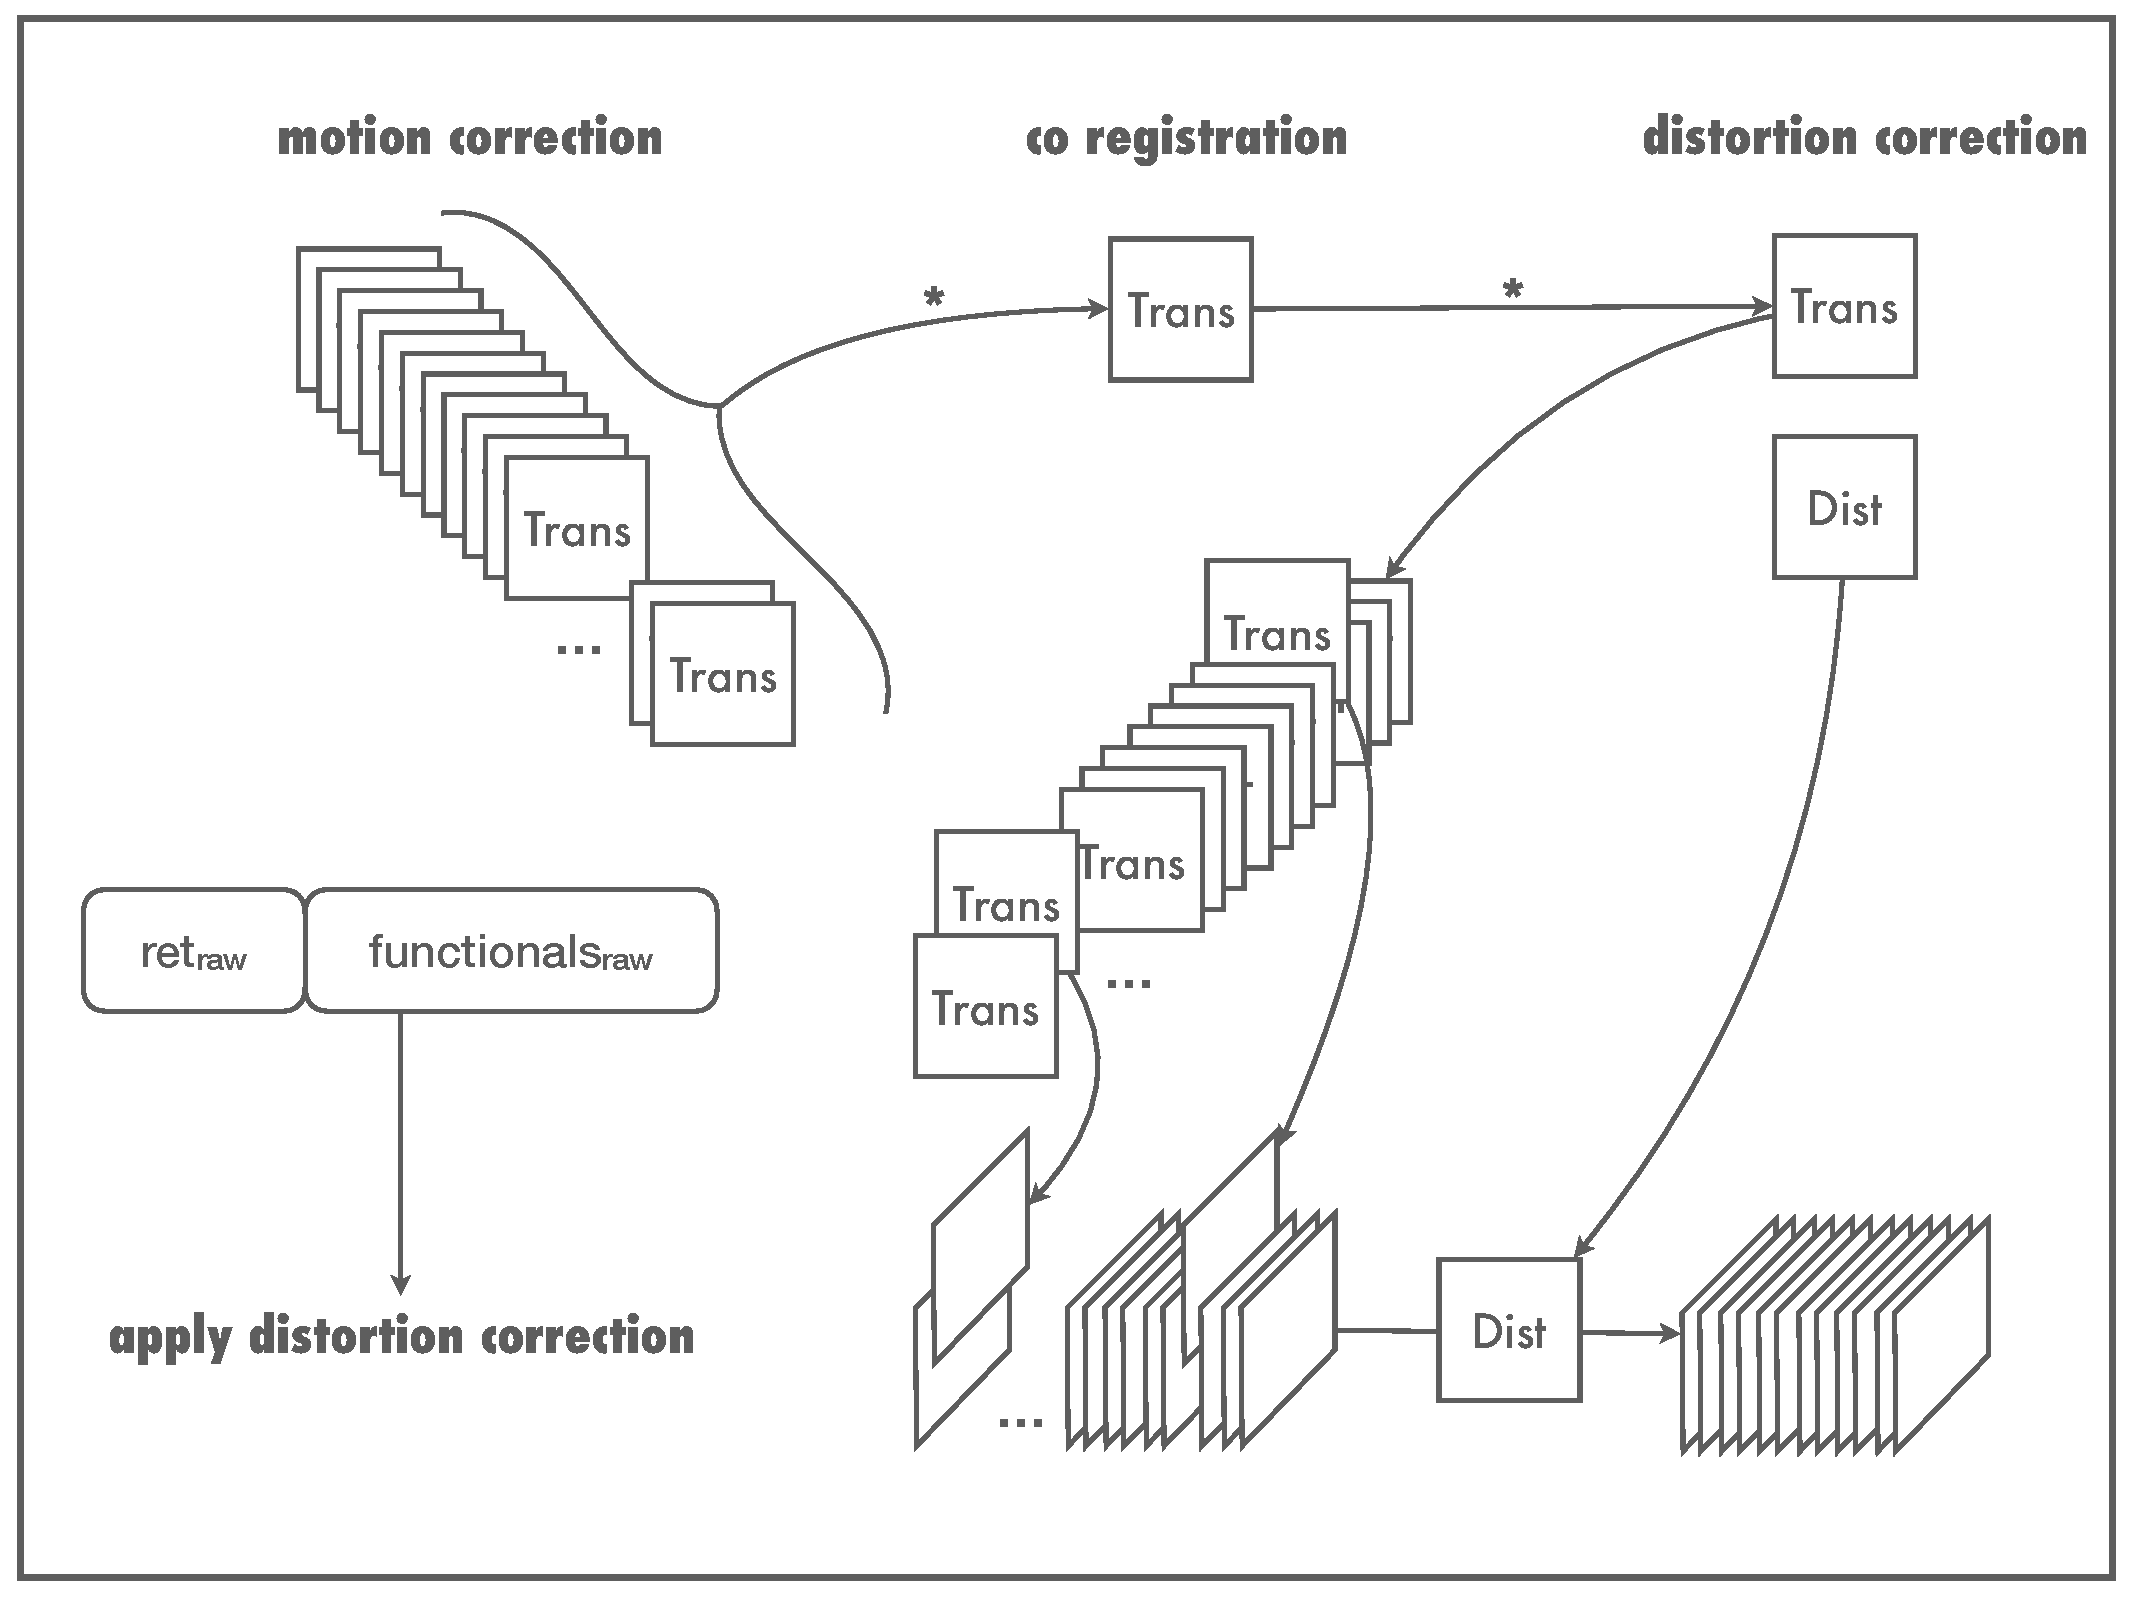
\includegraphics[width=0.8\textwidth]{applycorr}
\caption[Apply corrections from all steps at once]{Apply corrections from all steps at once}
\end{center}
\end{figure}

\FloatBarrier

\subsection{Retinotopy}
\begin{itemize}
\item sh runonqsub.sh 32gb do\_prepareretinotopy.sh 
\item sh do\_retinotopy.sh 256gb
\end{itemize}
\subsection{Functional laminar analysis}

\section{qsub}
You can run the respective scripts directly in a qsub instance:

\noindent When running the computation on the cluster use the wrapper function runonqsub.sh\\

\noindent \textbf{Important:}\\
\noindent runonqsub.sh does not work with do\_finecoregistration.sh (this function sets up a qsub session by itself). Please find more information below. The reason is that do\_finecoregistration.sh initiates a MATLAB session with the correct requirements and forwards this to qsub\\\\
\noindent the following requirements on memory and computation time can be expected:

\begin{table}[h]
\centering
\begin{tabular}{l | r | l}
\toprule
script & memory required & time required\\\hline
	do\_preparefunctionals.sh & 32GB & $\approx 10min$ \\\hline
	do\_fsrecon.sh & 16GB & $\approx 6h$ \\\hline
	do\_makemasksandlabels.sh & 16GB & $\approx 1min$ \\\hline
	do\_realignment.sh & 32GB & $\approx 30min$ \\\hline
	do\_preparecoregistration.sh & 16GB & $\approx 4.5h$ \\\hline
	do\_correctavgdiff.sh & 4GB & $\approx 3sec$ \\\hline
	do\_coregistration.sh & 8GB & $\approx 30min$ \\\hline
	do\_distcorr.sh & 32GB & $\approx 15min$ \\\hline
	do\_applydistcorr.sh & 64GB & $\approx 30min$ \\\hline
	do\_prepareretinotopy.sh & 32GB & $\approx 4min$ \\\hline
	do\_retinotopy.sh & 256GB & $\approx XXXmin$ \\\hline
	meanT.sh & 16GB & $\approx 2min$ \\\bottomrule
\end{tabular}
\caption[Approximated time and memory requirements when running on qsub]{Approximated time and memory requirements for the respective script to run. Note that everything that is more than 4GB must be run on the cluster. Use runonqsub.sh for that purpose.}
\label{tab:hardwarerequirements}
\end{table}

\newpage
\begin{figure}
\caption{Initial folder structure as required for the analysis}
\vspace{10pt}
{\footnotesize
\begin{forest}
  for tree={
    font=\ttfamily,
    grow'=0,
    child anchor=west,
    text height=0.15cm,
    parent anchor=south,
    anchor=west,
    calign=first,
    edge path={
      \noexpand\path [draw, \forestoption{edge}]
      (!u.south west) +(12pt,0pt) |- node[fill,inner sep=1.25pt] {} (.child anchor)\forestoption{edge label};
    },
    before typesetting nodes={
      if n=1
        {insert before={[,phantom]}}
        {}
    },
    fit=band,
    before computing xy={l=20pt},
  }
  [Analysis folder
[toolboxes/
    [analyzePRF-1.1/]
    [knkutils-master/]
    [OpenFmriAnalysis-master/]
    [spm12/]
    [vistasoft-master/]
  ]    
[S\#/ (set up by setupfolders.sh or when created using makenewsubject.sh)
  [0\_freesurfer/
  ]
  [1\_realignment/
  ]
  [2\_coregistration/
  ]
  [3\_distcorrection/
  ] 
  [4\_retinotopy/
  ]
  [5\_laminar/
  ]
  [A\_helperfiles/
    [acquisition\_parameters.txt]
    [b02b0.cnf]
    [b02b0\_example\_fsl.cnf]
    [RetStim.mat]
  ]
  [B\_scripts/
    [*.m]
    [*.sh]
  ]
  [C\_miscResults/
  ]
  [niftis/
  [functionals/]
  [inverted/]
  [pd/]
  [pdinverted/]
  [t1/]
  ]
]
[template\_session/
[template\_helperfiles/
	[acquisition\_parameters.txt]
    [b02b0.cnf]
    [b02b0\_example\_fsl.cnf]
]
[template\_scripts/
	[*.m]
    [*.sh]
]
]
[makenewsubject.sh]
]
\end{forest}

}
\label{tree:folderstruct}
\end{figure}

\FloatBarrier
\section{Helper files}
There are several helper files that are needed in order to perform the analysis:

\subsection{acquisition\_parameters.txt}
indicating the respective acquisition parameters per volume needed in order to perform the distortion correction. One line indicates the respective parameter setting for the respective volume (1st line corresponds to 1st volume, etc.)\\

\noindent e.g.:

\noindent 0 1 0 0.042\\
\noindent 0 -1 0 0.042\\

The first 3 columns indicate the respective phase coding direction the last column some weird value, that is only important if it changes. Otherwise it's fine to use any value as long as it is the same.

\subsection{b02b0.cnf}
Settings for distortion correction.

Needed in order to set the parameters for the distortion correction (example provided by FSL).

\subsection{RetStim.mat}
Stimuli used for retinotopy scans. Stimuli file must be such that each frame is represented as a binary image. The matrix must be of shape $Y \times X \times T$ where $X$ and $Y$ are the image dimensions in pixel and T is the respective number of frames. 

\section{Scripts explained (support for runonqsub.sh: Q)}
\subsection{runonqsub.sh}
Initiates a qsub session and sends it to the cluster. This is necessary, since scripts running on the cluster are copied to a different directory, but within scripts all directories are relative. runonqsub.sh must hence be run in a "normal" session not using qsub, giving the respective script that was intended to run as an argument. runonqsub will then set everything up correctly. Further you have to specify the amount of memory needed.\\

example: sh runonqsub.sh 32gb myscript.sh\\

Additional arguments can be passed after the script.\\

example: sh runonqsub.sh 16gb meanT.sh csfmask\\

Under the hood:
\begin{itemize}
\item a qsub session is initiated like so: qsub -l walltime=12:00:00,mem=\$1 -F "\$DIR \$\{@:3\}" \$DIR/\$2
\item \$DIR is the current absolute path to B\_scripts
\item \$1 is the amount of memory used (e.g. 32gb)
\item \$2 is the respective script to run (e.g. myscript.sh)
\item \$\{@:3\} is all following arguments that are parsed to the script
\item every time runonqsub.sh is called the absolute path is forwarded to the script (-F \$DIR) in order to keep the relative dependencies clear
\end{itemize}

\subsection{cleanscriptsfolder.sh}
Since qsub puts a output + error log into /B\_ scripts cleanscriptsfolder.sh can be used to move all qsub outputs to /B\_scripts/qsuboutput\\

\subsection{makenewsubject.sh}
executable script (double click to execute)\\

Creates a new subject (S\#) folder structure in order to get all folder dependencies right. It automatically detects folders called "S\textit{number}" and creates a new folder incrementing \textit{number} by one

\subsection{setupfolders.sh (Q)}
Sets up the necessary folder structure for the analysis (within a subject folder). This function is automatically called when using makenewsubject.sh\\

\noindent example: sh setupfolders.sh

\subsection{checkhelperfiles.sh (Q)}
Checks whether all necessary helper files are existing needed in order to perform the analysis.\\

\noindent example: sh checkhelperfiles.sh

\subsection{do\_preparefunctionals.sh (Q)}
Prepares functional data, i.e. removes the first 4 and the last x volumes of every set of functionals, where x is the number of volumes acquired after the stimulation ended. If files were modified (i.e. if volumes were deleted), the original file will remain in /niftis/functionals/old\\

\noindent example: sh do\_preparefunctionals.sh\\

\subsection{do\_fsrecon.sh (Q)}
Performs segmentation using Freesurfer.\\

\noindent If running on OSX the script assumes:\\
\noindent FREESURFER\_HOME=/Applications/freesurfer\\ 

\noindent If running on linux the script assumes:\\
\noindent FREESURFER\_HOME=/opt/freesurfer/version\\

\noindent The target image that is used for the segmentation must be located in /niftis/t1\\

\noindent example: sh do\_fsrecon.sh\\

\noindent Under the hood:
\begin{itemize}
\item calls recon-all -i /niftis/t1/* -subjid  0\_freesurfer -all
\item all results are stored in /0\_freesurfer
\end{itemize}

\subsection{do\_makemasksandlabels.sh (Q)}
example: sh do\_makemasksandlabels.sh\\

\noindent Uses FreeSurfer reconstruction to create masks for CSF, gray matter and white matter and creates labeled volume for use within retinotopy containing of left / right + gray / white matter.\\

\noindent If the orientation needs to be changed, parse the respective FreeSurfer compatible orientation parameter (\href{https://surfer.nmr.mgh.harvard.edu/pub/docs/html/mri_convert.help.xml.html}{https://surfer.nmr.mgh.harvard.edu/pub/docs/html/mri\_convert.help.xml.html})\\

\noindent example: sh do\_makemasksandlabels.sh RAS

\subsection{do\_realignment.sh (Q)}
example: sh do\_realignment.sh\\

\noindent Merges and motion corrects all files in /niftis/functionals using the average volume.\\

\noindent numberofvolumes.txt is written to /A\_helperfiles giving information about which sets had how many volumes. The first column is coresponds to dim4 from fslinfo\\

\noindent Opens an instance of fsleyes to show the results.\\

\noindent Under the hood:
\begin{itemize}
\item fslmerge is called to create a combined .nii for all files in niftis/functionals/ - files are merged allong the 4th dimension
\item a .txt file is created saving which files were merged and how many volumes were in there
\item mcflirt is used on the combined data doing the motion correction based on the mean volume
\item all results are stored in /1\_realignment
\end{itemize}

\subsection{do\_preparecoregistration.sh (Q)}
sets up mrVista session requirements, that is prepareing all files to be used with mrVista (defining Inplane anatomy, 3D Anatomy, functionals)\\

\noindent example: sh do\_preparecoregistration.sh

\subsection{do\_correctavgdiff.sh (Q)}
Due to the subtraction of the 1st from the 4th volume the area outside the brain has the highest value. In order to correct this the lowest value will be shifted to zero the a certain part of the higher values are cut (e.g. 0.975).\\

\noindent example: sh do\_correctavgdiff.sh 0.975\\

\noindent The result should be checked using "fsleyes ../2\_coregistration/Inplane/MCTemplate.nii.gz" to ensure that the area outside the brain is nulled. Note that it can happen that some areas within the brain are nulled as well. If they are not too wide spread they do not affect later coregistration.

\subsection{do\_coregistration.sh}
It will submit a qsub session using MATLAB, that in turn will be using FreeSurfer (bbregister) and OpenFmriAnalysis to perform a linear and non-linear boundary registration.  Movie files of the respective co-registration are stored in /C\_miscResults

\noindent The file used to execute MATLAB commands is /B\_scripts/do\_coregistration.m Note that it will be modified using the correct folder settings, which yields tmp.m that will be called and removed after MATLAB was closed.\\

example: do\_coregistration.sh

\subsection{do\_coregistration.m}
Sets up environment and initializes mrVista session. The function is used within do\_finecoregistration.sh.\\

Resulting transformation matrices (normal and inverted) are stored in /2\_coregistration\\

\subsection{do\_distcorr.sh (Q)}
example: sh do\_distcorr.sh\\

\noindent Uses the averge volume of the inverted set of images in /niftis/inverted as reference for \textit{inverted}\\

\noindent Uses as many volumes \textit{n} as there were in /niftis/inverted. Respective volumes are selected starting from the last going in \textit{4 x n} steps backward. Hence the resulting average of this set was computed over the 4th volume of each of \textit{n} last sets in the normal images. Simplified (all 1 are selected):\\

\noindent for n=5\\

\noindent 0,0,0,0,...,0,0,0,1,0,0,0,1,0,0,0,1,0,0,0,1,0,0,0,1\\

\noindent Both (normalavg and invertedavg) will be used to esimate the distortion correction.\\

\noindent Under the hood:
\begin{itemize}
\item reference volumes (normal + inverted) are selected in order to do the field distortion estimate (selection: see above).
\item selected reference volumes are merged into a single file (/3\_distcorrection/all\_b0.nii.gz)
\item topup is called using the merged (normal + inverted) .nii and performs field mapping accoriding to the specifications in /A\_helperfiles/b02b0.cnf using the acquisition parameters specified in acquisition\_parameters.txt
\item all results are stored in /3\_distcorrection
\end{itemize}

\subsection{do\_prepareapplytopup.sh (Q)}
Sets up files for use with do\_applydistcorr.sh \\

\noindent Motion correction and co-registration matrices are transformed into vector format (calling transmats2topup.sh). 

\noindent To each of the motion correction files the transformation from the coregistration and distortion correction is added. The actual addition is done in mergetransforms.sh \\

\noindent The result is a topup compatible file (first row zeros, second row actual transformation) for each volume.\\

\noindent The result will look like this:\\

\noindent $[0~0~0~0~0~0$ \\$Trans_x~Trans_y~Trans_z~Rot_x~Rot_y~Rot_z]$\\

\noindent Individual matrices for use with do\_applydistcorr.sh are stored in:\\

/2\_coregistration/transmatstoapply/\#\#\#\#.txt

\subsection{transmats2topup.sh}
Converts all transformation matrices contained within a specified folder to a 6 element vector having the following properties:\\

\noindent $[Trans_x~Trans_y~Trans_z~Rot_x~Rot_y~Rot_z]$\\

\noindent example: transmats2topup.sh $<$path relative to function$>$\\

\noindent The result of this transformation is stored in:\\

/$<$initial data folder$>$/topupformat/* \\

\noindent The wrapping is done using a MATLAB script (transmats2topup.m) running in the background. So since the function will load an instance of MATLAB in the background, inputting as many matrices as possible might be advisable.\\

\noindent Note that the function is called within do\_prepareapplytopup.sh

\subsection{transmats2topup.m}
Wrapper function to call tc\_transmat2vec.m for all files specified in the input. Since MATLAB is run in the background each call to a new function or script would initialize a new instance. By using this wrapper function MATLAB only has to be initialized once and processes all files in the respective input folder.

\subsection{tc\_transmat2vec.m}
A hack of the MATLAB function rotm2axang.m (Robotics toolbox), which per default transforms a set of 3x3 rotation matrices into single rotations around x,y and z. Additional functionality in tc\_transmat2vec.m includes readability for files compatible with dlmread.m Further the function outputs the translation. However it is necessary to supply a 4x4 transformation matrix or a string containing the filename of a file that is 4x4 transformation matrix in dlm readable format. The respective outcome is [axang,trans] with axang being the rotations around x,y,z in radians and trans being the translation along x,y,z

\subsection{mergetransforms.sh}
Adds input vector one element wise to input vector 2.\\

\noindent example: mergetransforms.sh file1.txt file2.txt\\

\noindent Note that the function is called within do\_prepareapplytopup.sh

\subsection{do\_applydistcorr.sh (Q)}
Applies distortion correction to all functional data.\\

\noindent example: sh do\_applydistcorr.sh\\

\noindent Under the hood:
\begin{itemize}
\item distortion correction is applied to the full set of functionals using the OUTPUT of topup (topup [$\ldots$] --out=OUTPUT) as well as acquisition\_parameters.txt (Using --method=jac)
\item all results are stored in /3\_distcorrection
\end{itemize}


\subsection{do\_prepareretinotopy.sh (Q)}
Prepares files for use with "do\_retinotopy.sh". The function copies all functionals to /4\_retinotopy and extracts the retinotopy volumes. A separate file containing those (ret.nii.gz) will be created in the respective folder. Afterwards a unzipped copy of "ret.nii.gz" will be created.\\

example: sh do\_prepareretinotopy.sh

\subsection{do\_retinotopy.sh}
Wrapper function to call a MATLAB script doing the retinotopic analysis (do\_retinotopy.m).\\

\noindent The functions submits a qsub MATLAB session to the cluster and runs the analysis. It can be specified how much memory to use.\\

example: sh do\_retinotopy.sh 32gb

\subsection{do\_retinotopy.m}
Computes retinotopic mapping. It uses /A\_helperfiles/RetStim.mat to obtain stimulus information and /4\_retinotopy/ret.nii as functional data file.

\subsection{meanT.sh (Q)}
example: sh meanT.sh my\_mask\\

\noindent Computes the averge activation per volume and outputs the respective result as "avgvolumeovertime.txt" in /C\_miscResults according to the region specified within the mask. If the function is called without pre-defined mask, the average over the full volume will be computed.\\

Masks can be csfmask, graymattermask, whitemattermask

\subsection{matmul.sh}
Matrix multiplication from files.\\

\noindent example: sh matmul.sh file1 file2

\subsection{multiply\_all\_M\_in\_A\_with\_B.sh}
Wrapper function that uses matmul.sh to multiply all matrices in the folder given in the first argument (path relative to function) and multiplies them with the matrix given in the second argument (path relative to function).\\

\noindent Note: the first argument (e.g. A) is a folder the second a file (e.g. B.txt).\\

\noindent example: sh multiply\_all\_M\_in\_A\_with\_B.sh A B.txt\\

\noindent The result of this transformation is stored in:\\

/$<$A$>$/matmulResults/* \\

\subsection{file2plot.sh}
Can be used to plot data from files.\\

example: sh file2plot.sh /C\_miscResults/avgvolumeovertimefullmask.txt

\subsection{liveupdateqsub.sh}
Submits a qstat -u user request every second.\\

example: sh liveupdateqsub.sh tomcla\\

\noindent exit command by hitting ctrl+c

\end{document}